\section{Physical Connections and Interfaces}

\begin{figure}[h]
\begin{center}
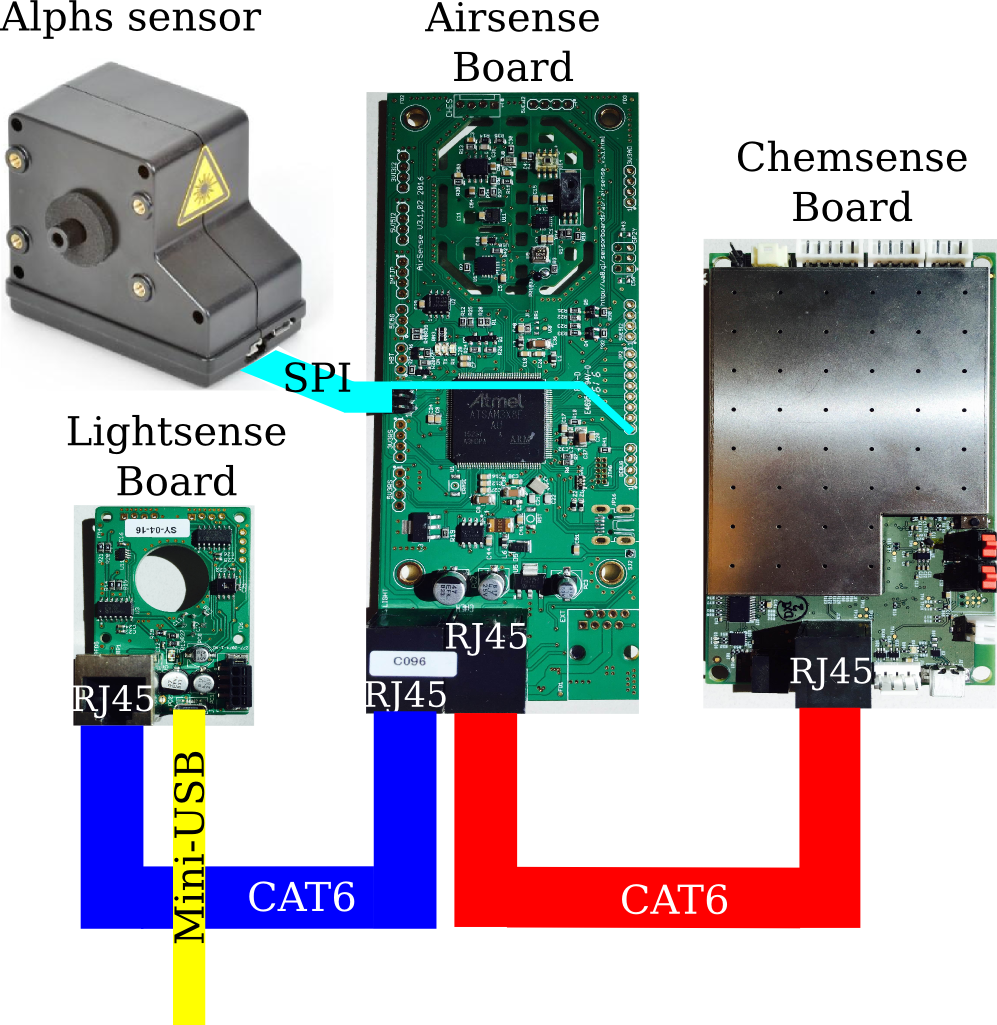
\includegraphics[width=4in]{physicalConnections.png}
\caption{Connections between the sensor boards and the sensor}
\label{fig:a}
\end{center}
\end{figure}


`v3 sensor boards with alpha sensor' means a set of sensors that are implemented on a v3.1 Metsense board, a v3.1 Lightsense board, and a Chemsense board and an independent alpha sensor.
\par
Physical connections between sensor boards and an alpha sensor are shown in the Figure \ref{fig:a}. A lightsense board and a chemsense board are connected to a metsense board through CAT6 cable. The metsense and the lightsense deliver data through I2C communication, and the chemsense board delivers data through serial3 communication. Alpha sensor is conncted to the metsense on SPI pins and one of GPIT pins. User requests and collects data from alpha sensor using SPI communication. All sensor data from metsense board, lightsense board, chemsense board, and alpha sensor are delivered to nodecontroller thourgh USB line attached on lightsense board using Serial communication. 
